\chapter{Analyse des besoins}


Comme on l'a vu dans l'approche théorique du \textit{Data Mining}, comme dans le cas de tout projet d'ailleurs, la définition des besoins est une étape cruciale du démarrage de l'activité. On va donc évoquer tout d'abord les besoins fonctionnels, puis les besoins non-fonctionnels.


\section{Besoins fonctionnels} 
Les besoins fonctionnels sont ceux qui permettent de remplir les conditions du cahier des charges ; ils sont incontournables. Il s'agit donc ici de voir comment on va répondre à la demande formulée à l'origine du projet. 
\iffalse
\section{Interface utilisateur}
%TODO: retravailler cette portion
L'interface utilisateur du programme sera composée d'un exécutable (\textit{dominionmining}minière de domination) qui sera exécuté avec certains paramètres pour réaliser l'action souhaitée. Le schéma ci-dessous représente les différentes interactions disponibles pour l'utilisateur:\\

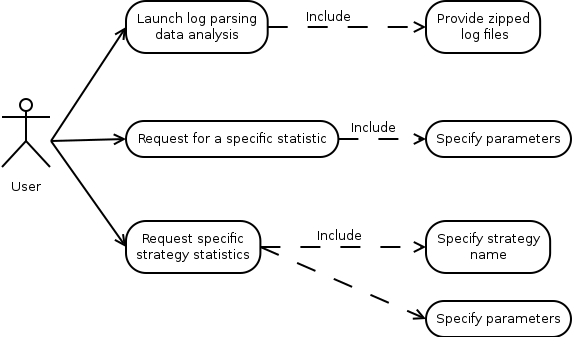
\includegraphics[scale=0.45,keepaspectratio]{diaRessources/UseCaseParsing}\\
Avant l'utilisation de toutes les fonctionnalités du programme, l'utilisateur doit lancer l'analyse.
\subsection{Lancement de l'analyse du log}
\subsubsection{Description et priorité}
\textbf{Niveau de priorité = haute}\\
\begin{itemize}
  \item L'utilisateur devra placer tous les logs compressés (fichiers tar.bz2) destinés à  être analysées dans un dossier spécifique.
  \item si aucune compression n'est donnée la compression par défaut est \textit{snappy}.
    \item Pour des fins de test, afin d'éviter d'avoir un 4 heures étape d'analyse, l'utilisateur peut spécifier un pourcentage des logs pour être analysée. en spécifiant une valeur comprise entre 0 et 100. l'analyseur choisira au hasard les logs de ceux qui sont prévus et les analyser, en créant une base de données utilisable pour des tests supplémentaires.
    \item Une fois que l'analyse est effectuée un message sera affiché sur la console (traitement de fait).

\end{itemize}

\subsection{Statistiques demandées}
\subsubsection{Description et priorité}
\textbf{Niveau de priorité = haute}\\
La demande d'une statistique peut être faite en tapant les états de \textit{dominionmining (paramètres)}.  \\
Les noms de stratégie possibles sont: big money, pen province, beyond silver.\\
Si d'autres stratégies sont reconnues par le programme, ils seront ajoutés à la liste.\\
La liste des paramètres qui seront possible d'utiliser sera déterminée dans le futur.\\

Le retour d'une statistique peut être un graphique affiché dans une fenêtre ou exportés vers un fichier. Si sa une valeur unique, un nom ou une phrase, il sera retourné à l'invite.

\subsection{Mappage des données de jeu}

Afin de permettre à l'utilisateur de demander des statistiques spécifiques concernant un jeu, le programme peut être exécuté afin de générer des logs de jeu simplifiées et un script python sera appliqué à ce log. Cela permettrait une plus grande flexibilité dans le type de statistiques affichables par le programme.
\begin{itemize}
\item Le programme sera lancé en utilisant la commande suivante: \textit{dominionmining data\_to\_query user\_script.py}
 \item Le script python sera appliquée au résultat généré et retourner les statistiques demandées par l'utilisateur.
\item Le fichier généré contenant les résultats de la requête aura le format suivant:
\begin{itemize}
\item Le nom du fichier produit est \textit{game.txt}
\item Le log simplifié contiendra chaque action effectuée par le joueur, une action par ligne. Liste des actions et leur format:
\begin{itemize}
\item Révéler une carte: \textit{joueur\_x révèle carte\_nom}
\item Piocher des cartes: \textit{joueur\_x jete n cartes}
\item Acheter une carte: \textit{joueur\_x buys carte\_name}
\item Jeter des cartes: \textit{joueur\_x trashes n cartes}
\item Mettre une carte \textit{joueur\_x puts carte\_name}
\item Gagner une carte: \textit{joueur\_x gains carte\_name}
\item Jouer une carte: \textit{joueur\_x jouer une carte\_name}

\end{itemize}
\end{itemize}
\end{itemize}
\fi
\subsection{Modélisation des données}
La première démarche consistait à modéliser les données disponibles pour créer une cohérence entre tous les formats existants. Il fallait commencer par décompresser les données, même si, comme on l'a vu, cela ne pouvait être fait que par "tranches" de temps (journées de \textit{Logs}) à cause des ressources mémoire disponibles. 

\subsubsection{Décompression des logs}
\paragraph*{Description et priorité} 



\textbf{Niveau de priorité = haute}



\begin{itemize}
  \item Les fichiers tar.bz2 seront stockés dans un dossier.
  \item Le programme va  décompresser un fichier spécifié à partir de ce dossier dans un dossier temporaire.
  \item Le programme va  supprimer les \textit{Logs} décompressés  à la demande du parser.
\end{itemize}

\subsubsection{Parser}

\paragraph*{Description et priorité} 



\textbf{Niveau de priorité = haute}



Compte tenu des problèmes mis en évidence en analysant un échantillon de \textit{Logs} (comme par exemple des incohérences de syntaxe), l'utilisation d'un parser (comme \textit{YACC} et \textit{LEX}) n'est pas recommandée. C'est pour cette raison que l'on va créer un parser qui utilisera les mots-clés et l'HTML déjà présents dans les \textit{Logs}. Ce parser sera responsable de la lecture et de la collecte des informations importantes sans perdre la structure du \textit{Log}.
Un aperçu des data devant être reconnues par le parser est représenté dans l'illustration suivante :\\


\includegraphics[scale=0.35,keepaspectratio]{diaRessources/UseCaseParser}

\begin{itemize}
\item Winners: liste des gagnants du jeu, il peut y avoir plusieurs gagnants en cas d'égalité.
\item Market: liste des 10 cartes disponibles pour être acheté par les joueurs.
\item Cards Gone: liste des cartes qui ont été entièrement acquises à la fin de la partie.
\item First hand: liste des cartes obtenues au début de partie.%à voir
\item Player Name: Nom du joueur.
\item Victory points: nombre de points à la fin de la partie.
\item Player cards: liste des cartes obtenues à la fin de jeu avec des noms et de quantités differents.
\item Victory cards: liste des cartes de victoire le joueur avec le acheté.
\item Trash: liste des cartes qui sont jetés à la fin de la partie.
\item Game Moves: liste des actions effectuées pendant chaque tour d'un joueur.
\end{itemize}
Le parser doit lire chaque élément montré dans le graphique précédent en tant que partie des données lorsque l'utilisateur exécute le programme de parsing\\

\subsubsection{Créer game-log}
\paragraph*{Description et priorité}
\textbf{Niveau de priorité = haute}\\
Cette fonctionnalité est la création d'une structure de données où les données du log seront écrites.
Voici une représentation graphique d'une vue d'ensemble de la structure de données:\\
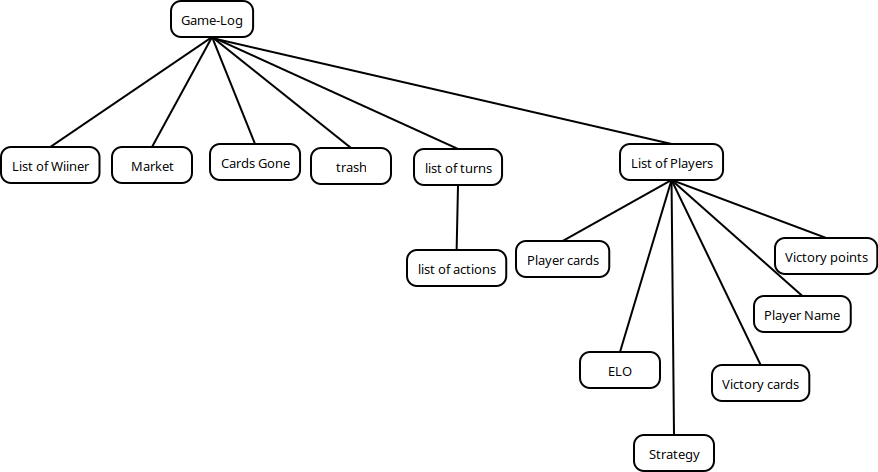
\includegraphics[scale=0.5,keepaspectratio]{diaRessources/game-log}

\subsubsection{Créer une base de données orientée document }

\paragraph*{Description et priorité}
\textbf{Niveau de priorité = haute}\\
Ce module sera responsable pour créer la base de données orientée document, contenant des données au format JSON.
\subsubsection{Se connecter à la base de données orientée document }
\paragraph*{Description et priorité}
\textbf{Niveau de priorité = haute}\\
\begin{itemize}
\item La base de données orientée document sera en charge des échanges à travers un socket spécifique.
\item La base de données orientée document recevra les logs de jeu au format JSON.
\item La base de données orientée document recevra les demandes du programme relatif à chaque élément de données qu'il contient.
\item La base de données orientée document enverra les résultats des demandes effectuées par le programme.
\end{itemize}


\subsubsection{Compression}
\paragraph*{Description et priorité}
\textbf{Niveau de priorité = moyen}\\

La base de données orientée document contiendra la plupart des données et un certain niveau de compression devra être appliquée.
La base de données que nous allons utiliser est focalisé sur mongodb, et il offre 2 niveaux de compression \textit{Zlib} et \textit{Snappy}.
Au cours du développement \textit{Snappy} est utilisé car il offre une meilleure performance.
Mais le programme final devrait donner à l'utilisateur la possibilité de choisir le niveau de compression lors du démarrage de l'analyse du log.

\subsubsection{Sauvegarder game-log}

\paragraph*{Description et priorité}
\textbf{Niveau de priorité = haute}\\
\begin{itemize}
\item La base de données orientée document permet de convertir la structure log de jeu dans un document au format JSON.
\item Les données fournies au format JSON seront stockées dans la base de données.
\end{itemize}
%partie de python à discuter
\subsection{Analyse des données}
\subsubsection{Recueillir des données}
\paragraph*{Description et priorité}
\textbf{Niveau de priorité = haute}\\
\begin{itemize}

\item L'analyseur de données va convertir les résultats de la requête dans un format utilisable par le module de plotting.
\item Si les données sont simples à lire (par exemple: un numéro, un nom, une phrase), l'analyseur de données sera tout simplement envoyer le résultat au format texte.
\item La dernière requête sera mémorisée avec son résultat afin de gagner du temps si la prochaine requête faite par l'utilisateur est le même.
\item Si l'utilisateur souhaite appliquer un script python de logs de jeu, le programme demandera les logs de jeu et les mettre dans un fichier texte, ce fichier contiendra chaque action faite par chaque joueur et le script sera appliqué à ce fichier.
\end{itemize}

\subsubsection{restorer game-log}
\paragraph*{Description et priorité}
\textbf{Niveau de priorité = moyen}\\

Cette fonction est responsable pour restaurer l'information manquante sur les logs analysés, en utilisant la déduction basique sur la base des données obtenues par le log.\\
En cas d'un en-tête du jeu manquant ou partie manquante:
  \begin{itemize}
\item Gagnants / cartes de victoire / points de victoire manquant: le programme peut garder la trace des cartes détenues par les joueurs pendant le jeu afin de savoir combien de cartes victoire qu'ils ont à la fin de la partie.
\item Market manquant: Le programme peut garder la trace des cartes achetées au cours du jeu afin de reconstituer partiellement ou totalement les cartes disponibles sur Market.
\item Cartes Gone: Comme avec les données manquantes de Market, le programme permet de garder une trace de cartes achetées et compter la quantité achetée pour chaque carte, si le montant maximum de cartes est acheté, la carte a disparu à la fin de la partie.
\item Nom du joueur manquant: le jeu se déplace partie d'un log assure également le suivi des noms des joueurs, le programme sera tout simplement de les restaurer dans l'en-tête.
\item Cartes de joueur: le programme permet de garder une trace des actions effectuées au cours du jeu par rapport aux cartes de joueurs et les ajouter dans cette liste.
  \end{itemize}

\subsubsection{Plotting}
\paragraph*{Description et priorité}
\textbf{Niveau de priorité = haute}\\

Le module de plotting va obtenir les données converties obtenues après le processus de recueillir des données et de les tracer dans une interface graphique. Ce module va fonctionner d'une manière similaire de \textit{GnuPlot}.

\subsubsection{Calculer l'\textit{\textbf{ELO}}}
%TODO
\subsubsection{Plotting}
\paragraph*{Description et priorité}
\textbf{Niveau de priorité = haute}\\

L'analyseur devra calculer la finale ELO pour chaque joueur et ce qui était un joueur ELO sur un jeu donné.
Pour chaque jeu dans l'ordre chronologique, ce module va demander au elo initiale des joueurs de la base de données relationnelle et les gagnants du jeu, puis il va calculer la nouvelle elo de chaque joueur de l'issue du jeu. Le module sera ensuite définir le elo calculés dans la base de données orientée documents au jeu en cours d'analyse et mettra également à jour l'elo globale pour chacun des joueurs qui participent au jeu sur la base de données relationnelle.\\

Plus d'informations sur ELO peuvent être consultés sur \url{https://en.wikipedia.org/wiki/Elo_rating_system}\\
\iffalse
%TODO: refaire le diagramme du calcul de l'elo
Le schéma suivant illustre le processus du calcul de elo:\\
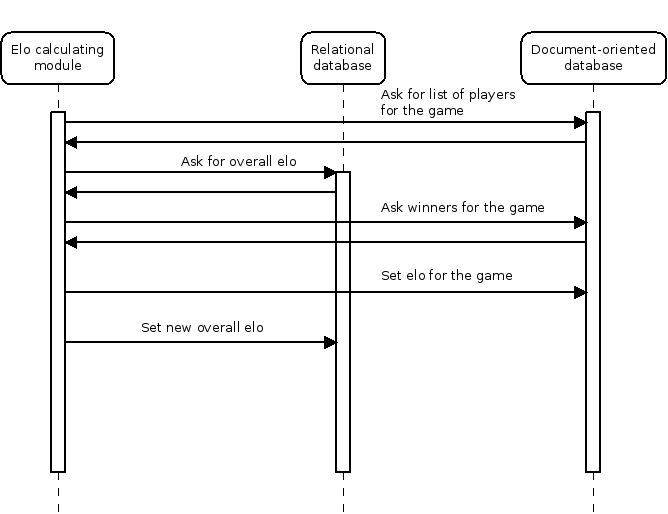
\includegraphics[width=\textwidth,height=\textheight,keepaspectratio]{diaRessources/elocalc}\\
\fi
\subsubsection{Reconnaître les stratégies}
\paragraph*{Description et priorité}
\textbf{Niveau de priorité = moyen}\\

Le wiki de dominion décrit quelques stratégies qui peuvent être utilisés dans le jeu.\\Par exemple :\\
Big Money\\
Beyond Silver\\
Penultimate Province Rule\\
Pour plus de détails sur \url{http://wiki.dominionstrategy.com/index.php/Strategy}\\



\textbf{Cette image décrit le processus de décision associé à la stratégie Big Money}\\
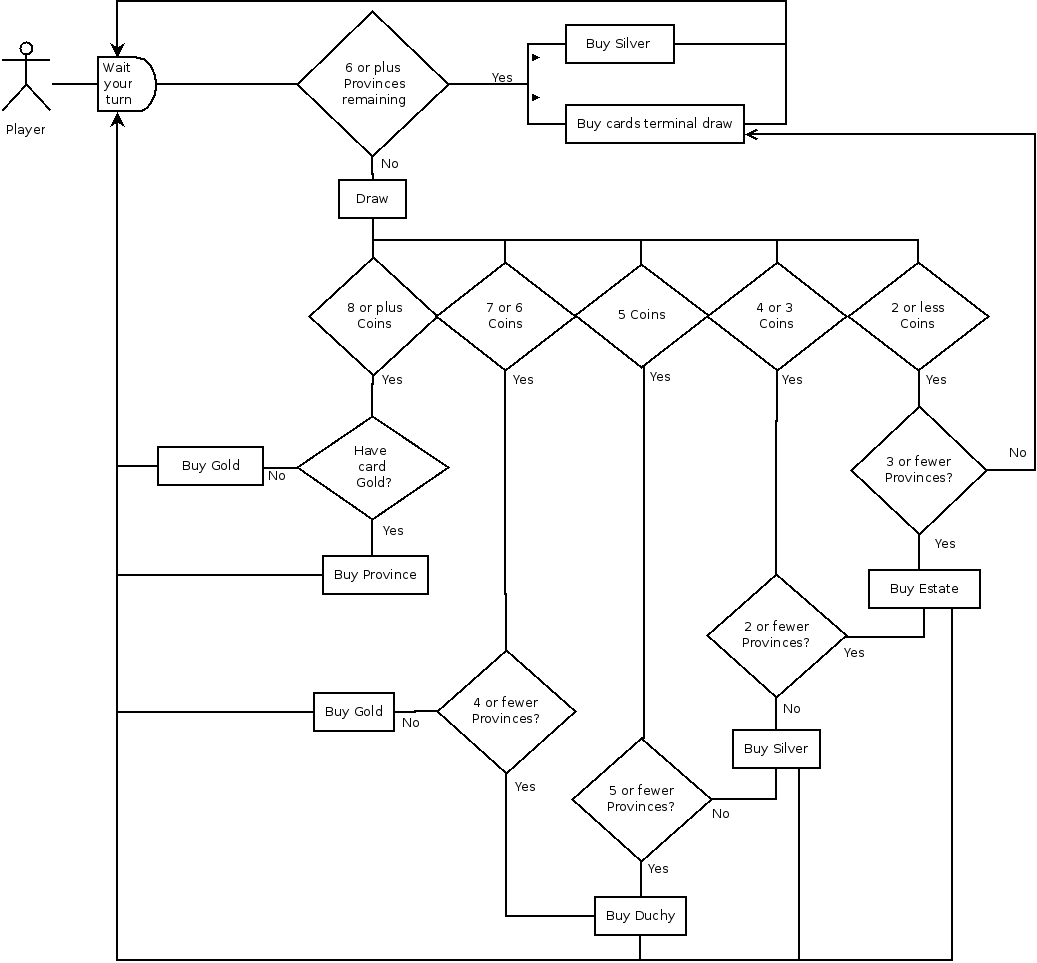
\includegraphics[width=\textwidth,height=\textheight,keepaspectratio]{diaRessources/big-money}\\
%The analyzer has to recognize when a player buys only money cards and specific cards related to the big money strategy. It also has to keep track of the remaining provinces to be bought.\\
Et l'analyseur devra être en mesure de reconnaître quelle stratégie a été utilisée sur un match donné (si une  stratégie a été utilisée) et générer des statistiques.\\
Plus de détails \url{http://wiki.dominionstrategy.com/index.php/Big_Money}\\

Afin de reconnaître la stratégie inventé Beyond Silver, l'analyseur doit reconnaître lorsque certains types de cartes sont achetées, la liste de ces cartes peuvent être trouvée sur : \url{http://wiki.dominionstrategy.com/index.php/Silver#Beyond_Silver}\\

Afin de reconnaître que Penultimate Province Rule est respecté (comme expliqué à \url{http://dominionstrategy.com/2011/03/28/the-penultimate-province-rule/}), l’analyseur doit garder une trace de la quantité de Points de Victoire de chaque joueur à chaque tour.

\subsubsection{Reconnaître le Greening}
\paragraph*{Description et priorité}
\textbf{Niveau de priorité = haute}\\

L'analyseur doit être capable de reconnaître le moment de \textit{\textbf{greening}} sur chaque match.
En savoir plus à propos de \textit{\textbf{greening}} sur \url{http://wiki.dominionstrategy.com/index.php/Greening}.\\
Le programme va reconnaître quand greening arrive en détectant lorsque les cartes de victoire commencent à être achetées.

\newpage

\section{Besoins non-fonctionnels}

\subsection{Besoins de performance}

Aucun besoin de performance spécifique n’a été fait par le client. Mais pour l'analyseur le temps d’exécution  doit être inférieur à une heure.\\
L'utilisateur doit être capable de parcourir le processus d'analyse sur un ensemble de données précis sans devoir attendre que la même requête à refaire.

\subsection{Fiabilité}

Le client demande que le nombre maximum de log doivent être analysé, que les données fournies ont des incohérences et quelques logs ne seront pas possibles d'analyser.\\
L'analyseur devra analyser 100\% des données présentes sur le log et restaure toute information manquante si possible.\\
\subsection{Attributs de qualité de logiciels}

Même si seulement une ligne de commande est prévue pour le programme final, elle devrait avoir une courbe facile à apprendre et être facile à utiliser.\\
Les données générées par l'analyseur n’ont pas besoin à être lisibles par l'homme.\\
Les game log générés devront être analysés par l'utilisateur afin de permettre la plus grande souplesse possible dans le traitement des logs.

\section{Besoins organisationnels}

La répartition des tâches du projet et l'estimation de la durée de chacune d'elle sont présentées sur le planning suivant:\\

\subsection{Planning prévisionnel}

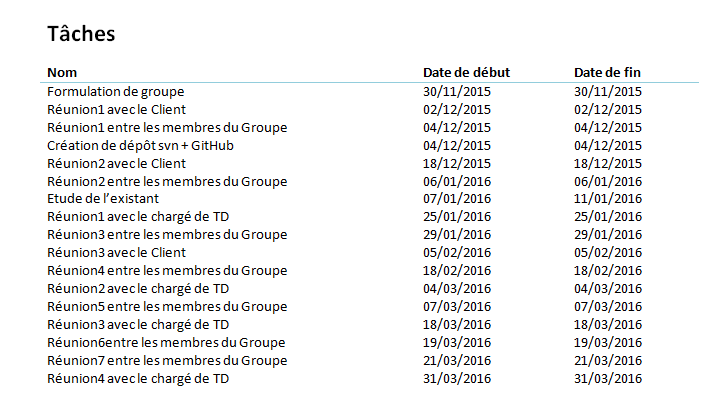
\includegraphics[scale=0.45,keepaspectratio]{planning}\\

\subsection{Diagramme de Gantt}

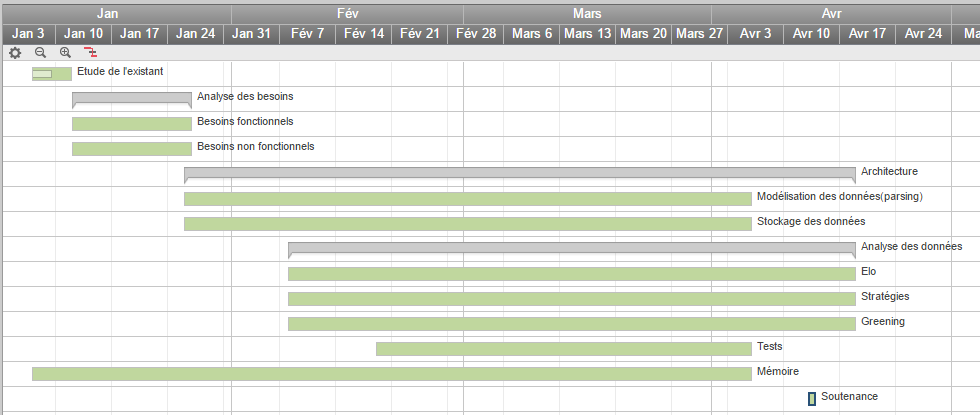
\includegraphics[scale=0.45,keepaspectratio]{gantt}\\

\newpage

\section{Développement}

Intro

\subsection{Tâches}

Bla\\


%tableau à taille fixée sur certaines colonnes (param sur la ligne \begin{tabularx}, voir wiki pour plus d'info sur la syntaxe
\begin{figure}[!h]
\begin{center}
\begin{tabularx}{17cm}{|c|p{6cm}|X|}
  \hline
  Priorité & Nom & Raison\\
  \hline
  1 & Tache 1 & Doit être vérifié en premier car sinon [...] \tabularnewline
  2 & Tache 2 & On doit pouvoir [...] \tabularnewline
  3 & Tache 3 & Comme les principales fonctionnalités permettant de tester sont opérationnelles, nous pouvons passer à cette tâche. \tabularnewline
  4 & Tache 4 & Parce que [...] \tabularnewline
  5 & Tache 5 & La tache 5 fait partie des principales [...]. \tabularnewline
  6 & Tache 6 & Dernière fonctionnalité essentielle à mettre en place. \tabularnewline
  7 & Tache 7 & Non-essentiel, mais apporterait un plus au projet. \tabularnewline
  8 & Tache 8 & Non-essentiel, mais apporterait un plus au projet. \tabularnewline
  \hline
\end{tabularx}
\end{center}
\caption{Tableau récapitulatif des tâches}
\end{figure}

\subsection{Tests}

Bla\\

\begin{figure}[!h]
\begin{center}
\begin{tabularx}{17cm}{|p{6cm}|X|}
  \hline
  Fonctionnalité & Test\\
  \hline
  Fonction 1 & Quand [...], vérifier [...]. \tabularnewline
  & Et quand [...], vérifier [...]. \tabularnewline
  Fonction 2 & Vérifier [...]. \tabularnewline
  Fonction 3 & Vérifier [...]. \tabularnewline
  Fonction 4 & Avoir [...]. \tabularnewline
  Fonction 5 & Accéder à [...]. \tabularnewline
   & Vérifier que [...]. \tabularnewline
  Fonction 6 & Accéder à [...]. \tabularnewline
   & Et vérifier [...]. \tabularnewline
  Fonction 7 & Installer [...]. \tabularnewline
   & Vérifier [...]. \tabularnewline
  Fonction 8 & Compter [...]. \tabularnewline
  \hline
\end{tabularx}
\end{center}
\caption{Tableau récapitulatif des tests}
\end{figure}
